\setcounter{section}{4}
\setcounter{subsection}{16}
\subsection{IPv6 in Wireshark}

Analysieren Sie das zur Verf"ugung gestellte Wireshark-Capture. Zeigen Sie,
\begin{enumerate}[(a)]
    \item welche Werte im 'Next Header'-Feld auftreten.

        Das „Next Header“-Feld gibt an, welches Protokoll im nächsten Abschnitt
        des Pakets verwendet wird.

        Beispiele hierzu finden sich in den Abbildungen \ref{fig:4.17.a.1}
        (ICMPv6) und \ref{fig:4.17.a.2} (TCP)

    \item wie lang die verwendeten Adressen sind und welche Werte diese annehmen

        IPv6-Adressen sind 128-Bit lang. Es gibt
        \begin{itemize}
            \item Unicast-Adressen
                \begin{itemize}
                    \item Global Unicast, \verb|2000::/3|; routbar und im Internet erreichbar.
                    \item Link-Local -- \verb|FE80::/10|; nur für dieselbe Verbindung verwendet, nicht routbar im Internet.
                    \item Loopback -- \verb|::1/128|; an eine Loopback-Adresse gesendete Pakete werden auf derselben Schnittstelle zurückgesendet.
                    \item Unique Local -- \verb|fc00::/7|; nur im Rahmen privater Netze routbar, nicht aber im globalen IPv6-Internet
                    \item IPv4-in-IPv6 -- \verb|::/80|; IPv4-kompatible oder IPv4-gemappte IPv6-Adresse.
                    \item Unspecified -- \verb|::/128|;
                \end{itemize}
            \item Multicast-Adressen
                \begin{itemize}
                    \item Alle Knoten -- \verb|FF02::1|;
                    \item Alle Router -- \verb|FF02::2|;
                    \item DVMRP Router -- \verb|FF02::4|;
                    \item OSPFv3 SPF Router -- \verb|FF02::5|;
                    \item OSPFv3 DR Router -- \verb|FF02::6|;

                        ...
                \end{itemize}
            \item Anycast-Adressen

                sind Unicast-Adressen, die absichtlich mehreren
                Schnittstellen zugewiesen wird, sodass der Datenverkehr stets
                an die topologisch nächstgelegene Instanz geleitet wird.
        \end{itemize}

    \item auf wen die verwendeten IPv6-Adressen registriert sind.

        Wir betrachten die Destination-Adresse \verb|2001:6f8:900:7c0::2| (siehe Abbildung~\ref{fig:4.17.c.1})

        Die Ausgabe des \verb|whois|-Tools unter Linux zeigt die relevanten
        Informationen zur Adresse, wem die Adresse gehört.

\begin{verbatim}
> whois 2001:6f8:900:7c0::2

% This is the RIPE Database query service.
% The objects are in RPSL format.
%
% The RIPE Database is subject to Terms and Conditions.
% See https://docs.db.ripe.net/terms-conditions.html

% Note: this output has been filtered.
%       To receive output for a database update, use the "-B" flag.

% Information related to '2001:6f8:800::/39'

% Abuse contact for '2001:6f8:800::/39' is 'abuse@gtt.net'

inet6num:       2001:6f8:800::/39
netname:        EASYNET-DE-ALLOC
descr:          Easynet Germany Allocation
country:        DE
admin-c:        RG-RIPE
tech-c:         EDEN-RIPE
tech-c:         ENH66-RIPE
mnt-by:         EASYNET6-MNT
mnt-lower:      EASYNET6-MNT
status:         ALLOCATED-BY-LIR
created:        2002-08-06T16:54:38Z
last-modified:  2008-12-02T15:10:00Z
source:         RIPE

role:           Easynet Germany NOC
address:        Easynet GmbH
address:        Nagelsweg 33-35
address:        20097 Hamburg
address:        Germany
phone:          +49 180 44746624
fax-no:         +49 180 5003087
admin-c:        RG-RIPE # Robert Gutknecht
tech-c:         ULF-RIPE # Ulf Fischer
nic-hdl:        EDEN-RIPE
remarks:        operation of the Easynet Germany backbone
mnt-by:         EASYNET-DE-MNT
created:        2003-01-04T01:17:16Z
last-modified:  2015-09-09T11:18:48Z
source:         RIPE # Filtered

role:           Easynet IPv6 Hostmaster
address:        Easynet Network Operations Centre
address:        Easynet Group PLC
address:        5 Thomas More Square
address:        London E1W 1YW
address:        England
address:        GB
phone:          +44 20 7 032 5200
fax-no:         +44 20 7 032 5335
admin-c:        PPD-RIPE  # Phil Duffen
admin-c:        SOM-RIPE  # Soenke Mumm
admin-c:        ULF-RIPE  # Ulf Fischer
tech-c:         PPD-RIPE  # Phil Duffen
tech-c:         SOM-RIPE  # Soenke Mumm
tech-c:         ULF-RIPE  # Ulf Fischer
nic-hdl:        ENH66-RIPE
mnt-by:         EASYNET6-MNT
created:        2002-07-13T12:02:22Z
last-modified:  2011-10-25T12:42:26Z
source:         RIPE # Filtered

person:         Robert Gutknecht
address:        Plusserver GmbH
address:        Nagelsweg 33-35
address:        20097 Hamburg
address:        Germany
phone:          +49 40 771750
fax-no:         +49 40 77175519
nic-hdl:        RG-RIPE
mnt-by:         NEXINTO-MNT
created:        2002-07-29T09:42:28Z
last-modified:  2018-12-06T13:47:39Z
source:         RIPE # Filtered

% Information related to '2001:6f8::/32AS3257'

route6:         2001:6f8::/32
descr:          GTT
origin:         AS3257
mnt-by:         AS3257-ROUTE-MNT
created:        2022-03-09T07:58:27Z
last-modified:  2022-03-09T07:58:27Z
source:         RIPE

% This query was served by the RIPE Database Query Service version 1.117 (DEXTER)
\end{verbatim}

    \item wie lang die maximale 'Payload Length' ist

        1452 (siehe Abbildung~\ref{fig:4.17.d.1})

\end{enumerate}

\begin{figure}[p]
    \centering
    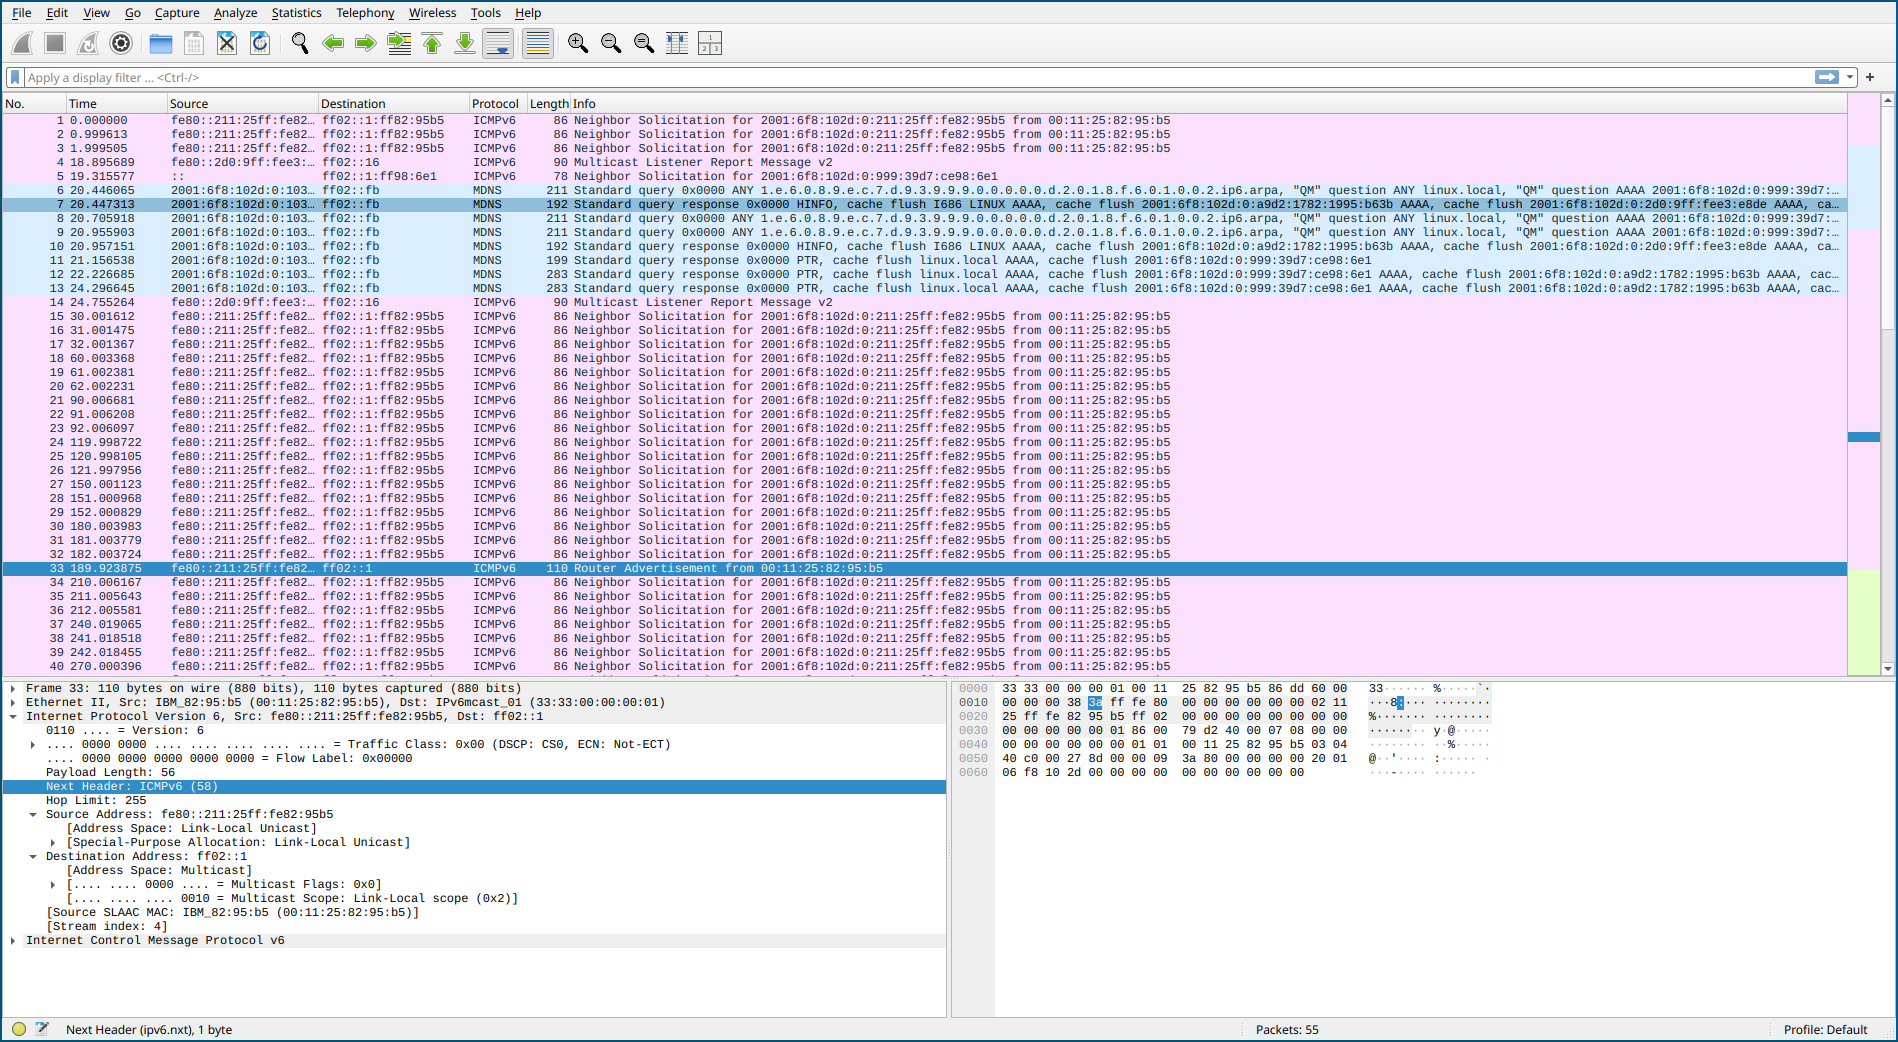
\includegraphics[width=1\textwidth]{./assets/4.17.a.1.png}
    \caption{}
    \label{fig:4.17.a.1}
\end{figure}

\begin{figure}[p]
    \centering
    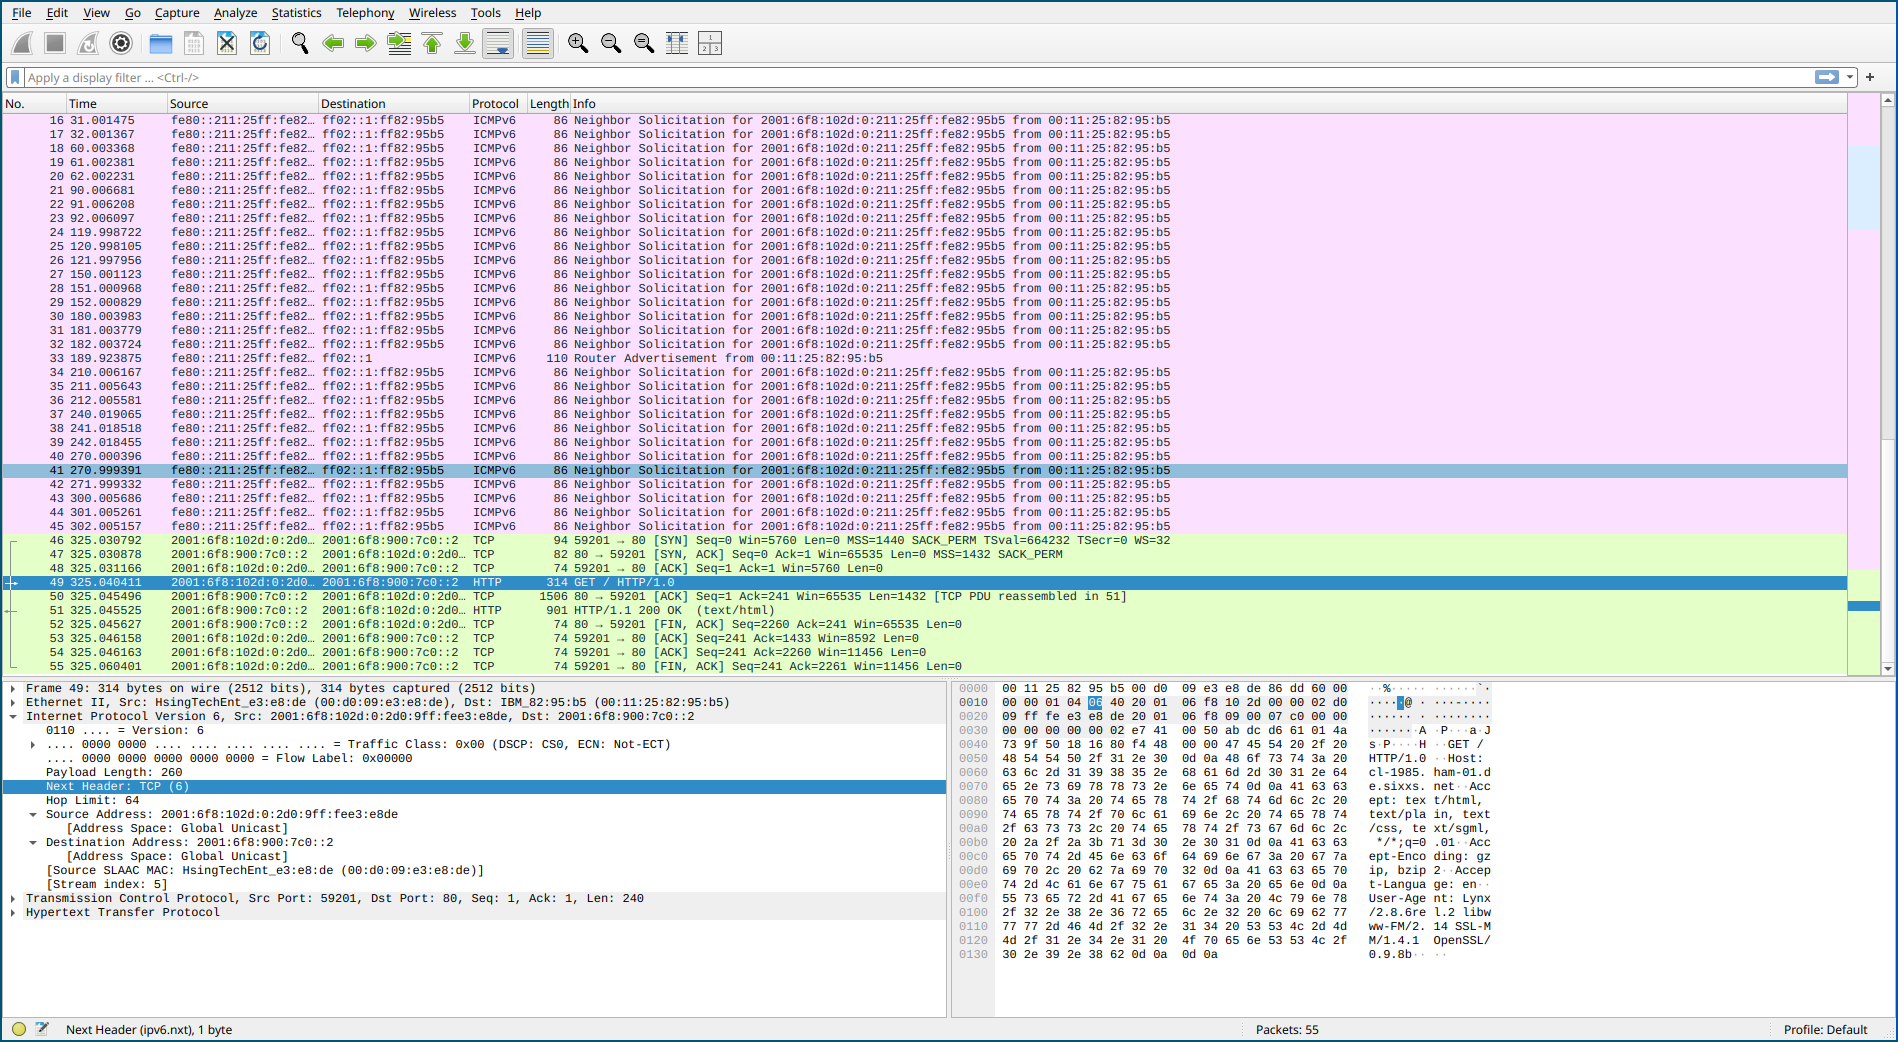
\includegraphics[width=1\textwidth]{./assets/4.17.a.2.png}
    \caption{}
    \label{fig:4.17.a.2}
\end{figure}

\FloatBarrier

\begin{figure}[p]
    \centering
    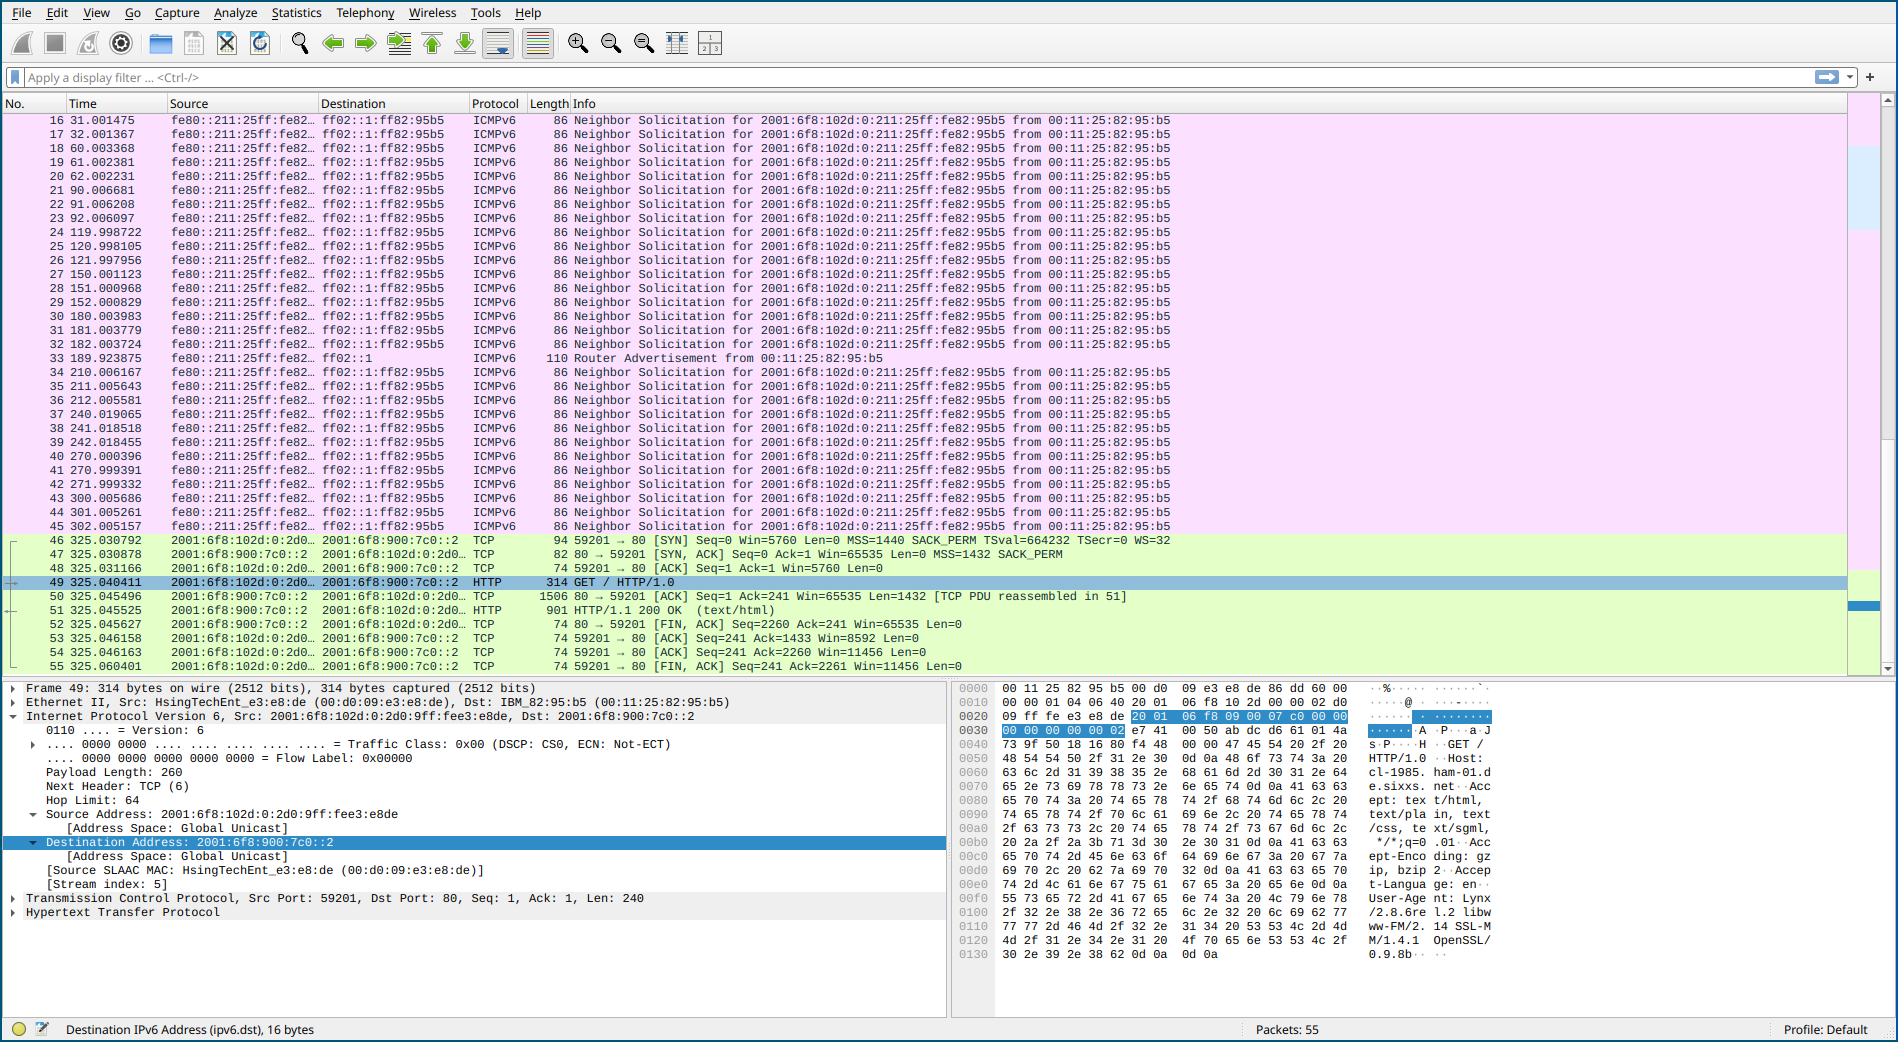
\includegraphics[width=1\textwidth]{./assets/4.17.c.1.png}
    \caption{}
    \label{fig:4.17.c.1}
\end{figure}

\begin{figure}[p]
    \centering
    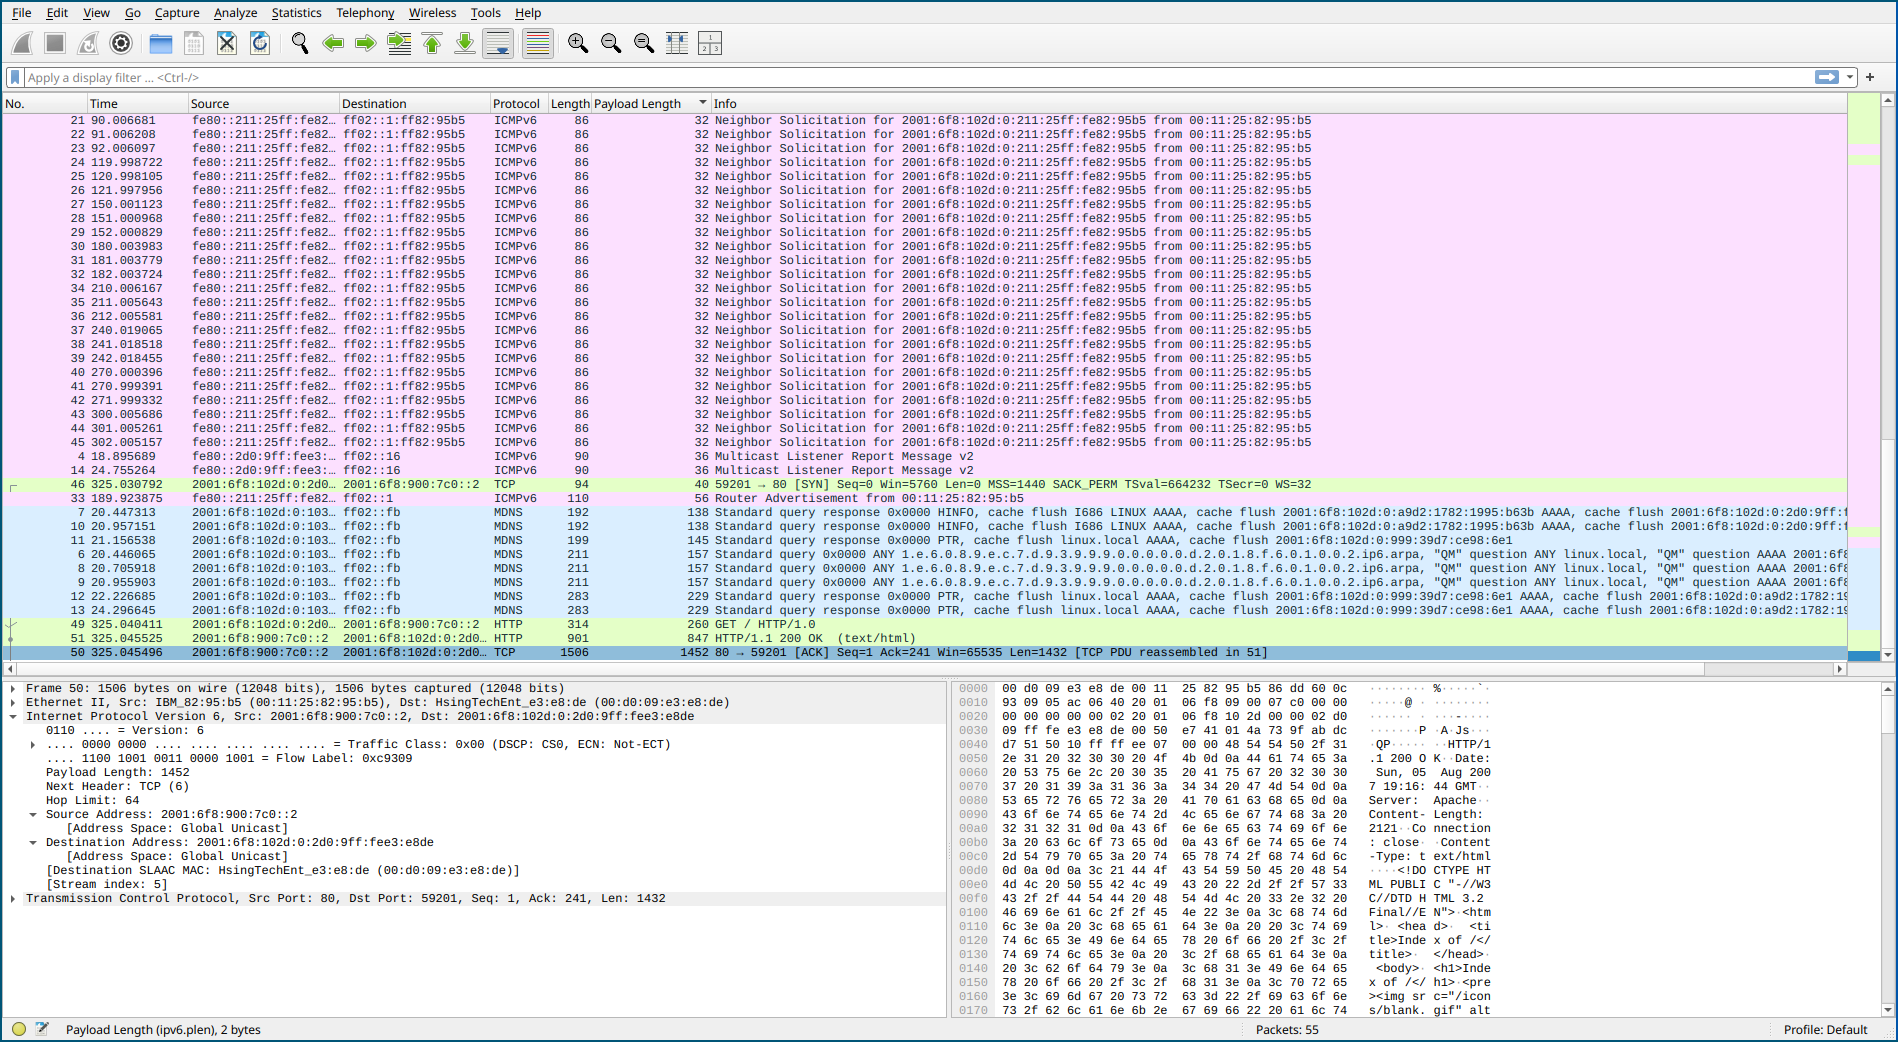
\includegraphics[width=1\textwidth]{./assets/4.17.d.1.png}
    \caption{}
    \label{fig:4.17.d.1}
\end{figure}

\FloatBarrier
